\documentclass[a4paper,11pt,oneside]{scrreprt}
\usepackage[latin1]{inputenc}
\usepackage[english]{babel}
\usepackage{graphicx}
\usepackage{float}
\usepackage{geometry}
\geometry{verbose,a4paper,tmargin=25mm,bmargin=25mm,lmargin=15mm,rmargin=25mm}
\usepackage{paralist}

\usepackage{paracol}

\usepackage{todonotes}

\usepackage{listings}
\lstset{language=Java,
	tabsize=2,
	showspaces=false,
	showtabs=false,
	breaklines=true,
	showstringspaces=false,
	breakatwhitespace=true,
	commentstyle=\color{pgreen},
	keywordstyle=\color{pblue},
	stringstyle=\color{pred},
	basicstyle=\footnotesize\ttfamily,
	moredelim=[il][\textcolor{pgrey}]{$$},
	moredelim=[is][\textcolor{pgrey}]{\%\%}{\%\%}
}

\usepackage{tikz}
\usetikzlibrary{calc,patterns,angles,quotes}

\usepackage{caption}
\usepackage{subcaption}
\usepackage{tabularx} % in the preamble

\begin{document}


\begin{center}
	Submitted by Group 51
	
	\bigskip
	
	\begin{tabular}{c}
	Group Members: \\
	CETIN, Ulfet (391819); GRUCZKA, FILIP (413279);	LIPINSKI, Bartosz (413177) \\
	\end{tabular}

	\bigskip
	
	DIS1 WS 19/20 Assignment 4\\
	Types of Knowledge and Mistakes
	
	%	(ordered on lastname basis)
\end{center}

\section*{Task 1}

\begin{tabularx}{\textwidth}{|X|}
	\hline
	\textbf{Knowledge in the World and Knowledge in the Head}\\
	\hline
	Instances of Knowledge in the World from the Video:
	
	\begin{itemize}
		\item alpha 
		\item beta
		\item gamma
	\end{itemize}

	\\
	\hline
	Instances of Knowledge in the Head from the Video:
	
	\begin{itemize}
		\item alpha 
		\item beta
		\item gamma
	\end{itemize}
	
	\\
	\hline
%	\raisebox{-\height}[0pt][0pt]{
\includegraphics[clip, trim=0cm 0cm 0cm 0cm, scale=0.2]{./images/redesign.png} }
	
\end{tabularx}\\

	Redesign:\\
	
\begin{figure}[h]
	\centering
	
\includegraphics[clip, trim=0cm 0cm 0cm 0cm, scale=0.25]{./images/redesign.png}
\end{figure}

	Explanation:\\
	

\bigskip


%\begin{figure}[h]
%	\centering
%	\includegraphics[clip, trim=0cm 7cm 29cm 0cm, scale=0.5]{./images/bad1st.png}
%	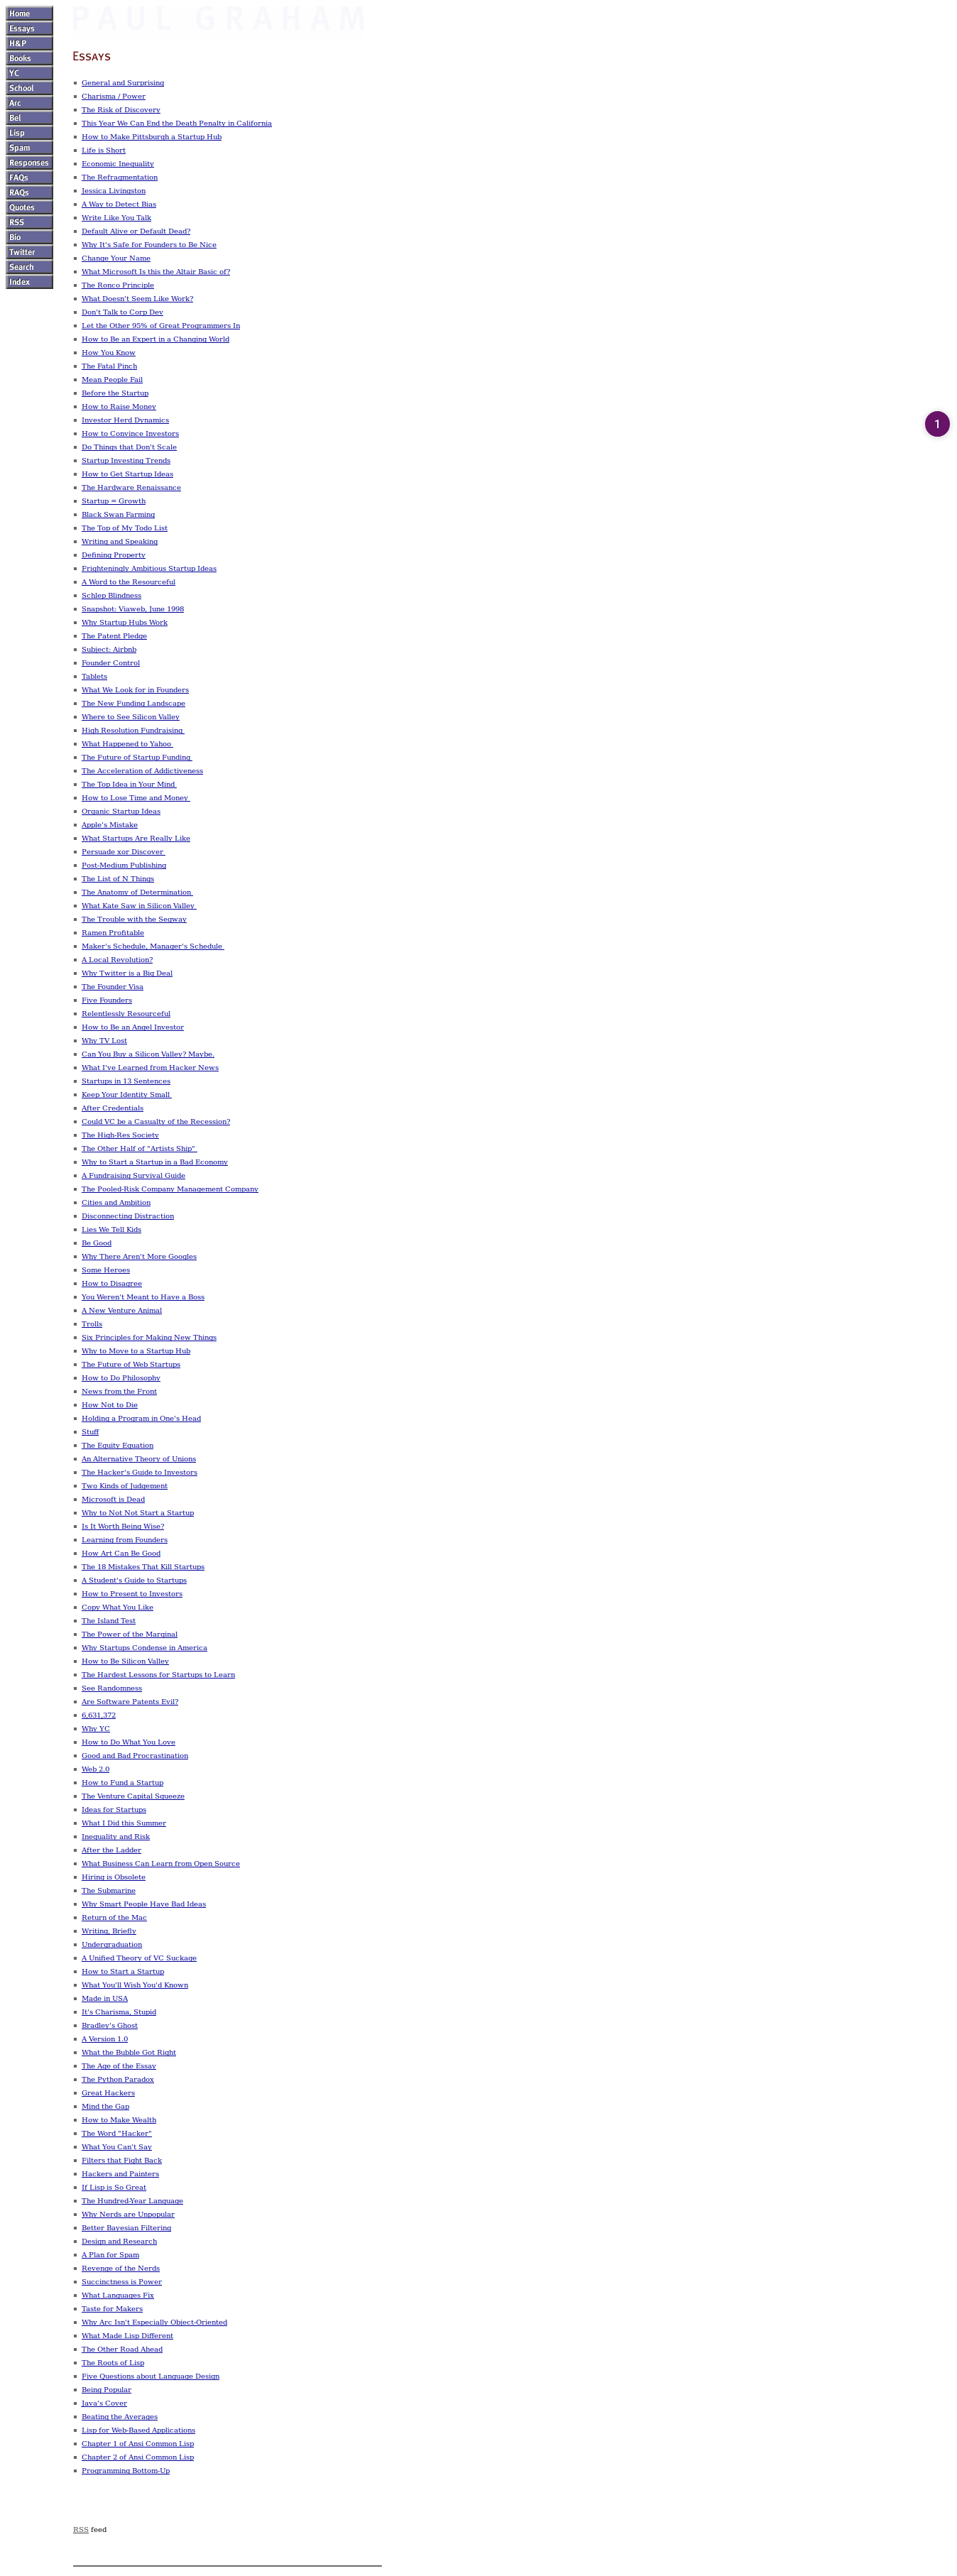
\includegraphics[clip, trim=0cm 113cm 29cm 0cm, scale=0.5]{./images/bad2nd.png}
%\end{figure}
%

%\begin{figure}[H]
%	\centering
%	\begin{subfigure}{.5\textwidth}
%		\centering
%		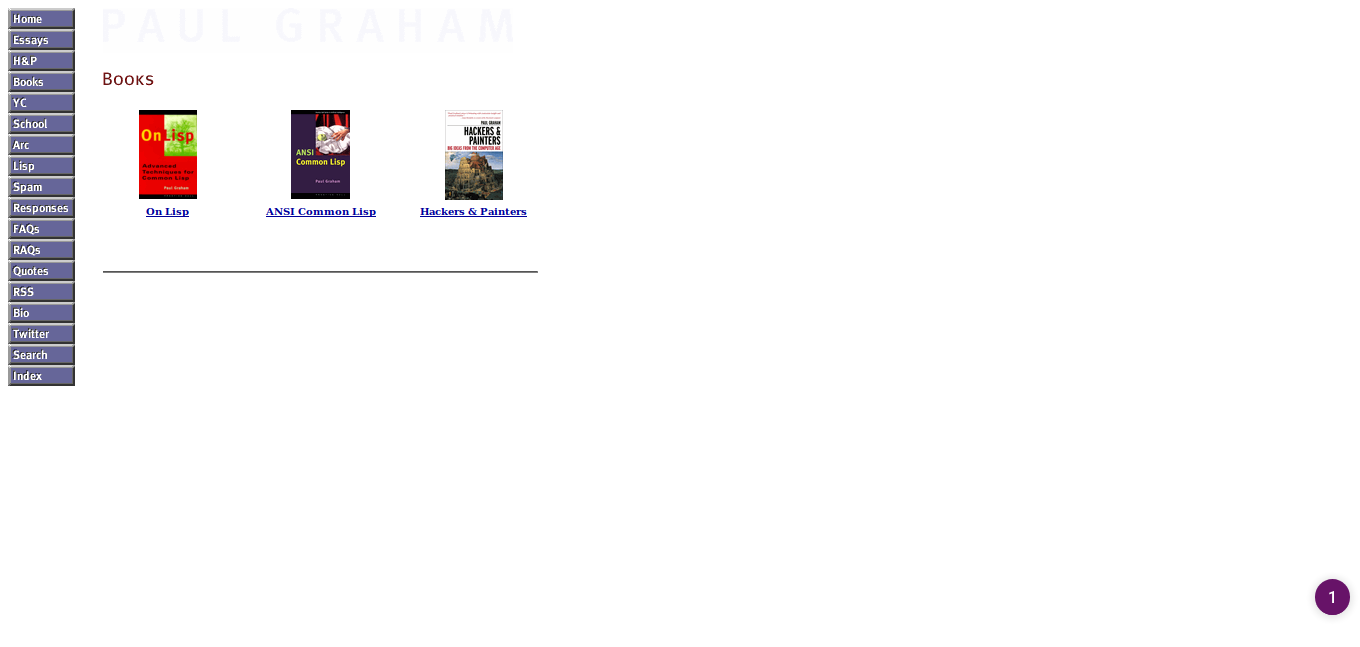
\includegraphics[clip, trim=0cm 7cm 25cm 0cm, scale=0.5]{./images/bad3.png}
%%		\caption{A subfigure}
%		\label{fig:sub1}
%	\end{subfigure}%
%	\begin{subfigure}{.5\textwidth}
%		\centering
%		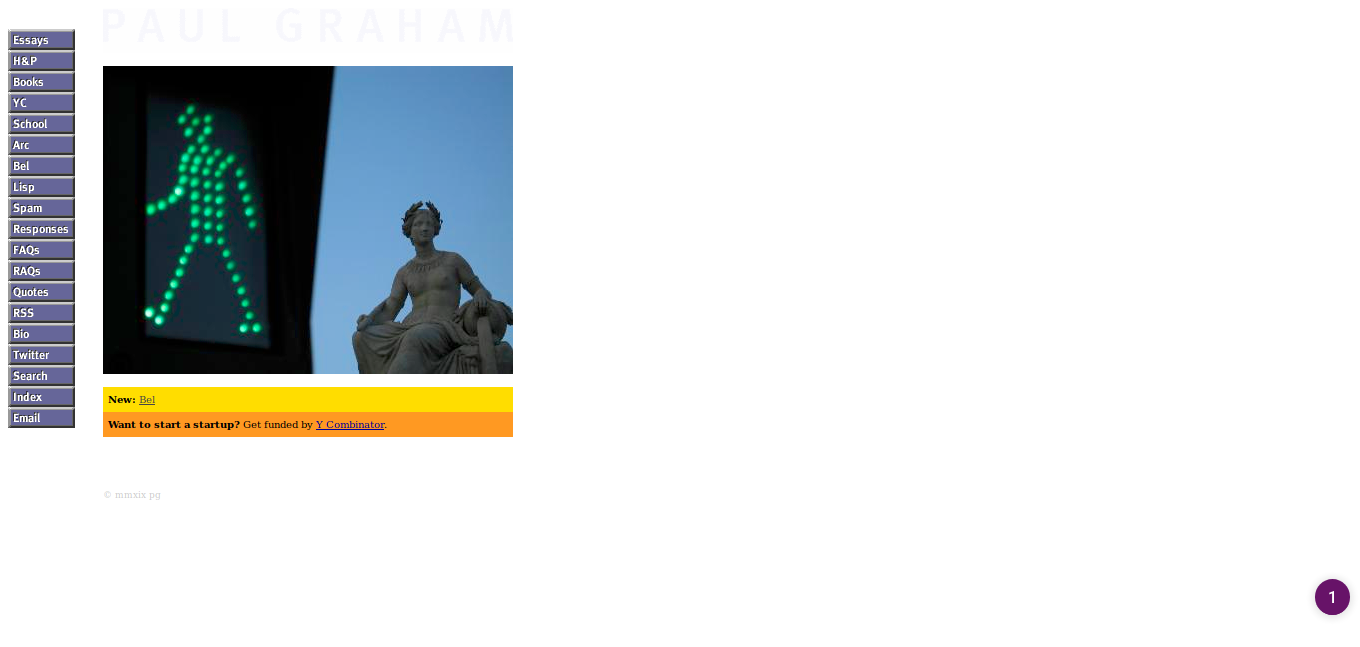
\includegraphics[clip, trim=-2cm 7cm 25cm 0cm, scale=0.50]{./images/bad1.png}
%%		\caption{A subfigure}
%		\label{fig:sub2}
%	\end{subfigure}
%	\caption{Paul Graham website}
%	\label{fig:test}
%\end{figure}
\clearpage

\section*{Task 2}

\begin{tabularx}{\textwidth}{|X|}
	\hline
		\textbf{Mistakes}
		\\
	\hline
		\textbf{Task:}
		\\
	\hline
		\textbf{Mistake:}
		
		\\
		
		\textbf{Cause:}
		\\
	\hline
		\textbf{Redesign:}
		
		\\
		
		\textbf{Explanation:}
		
			\begin{compactenum}[	a)]
				\item How the redesign minimizes the implications of the mistake:
				\item How the redesign minimizes the chances of the mistake occurring in the future:
			\end{compactenum}
	\\
	\hline
	
	
	
	%	\raisebox{-\height}[0pt][0pt]{
\includegraphics[clip, trim=0cm 0cm 0cm 0cm, scale=0.2]{./images/redesign.png} }
	
	%	\hline
	
\end{tabularx}\\

\end{document}}
